\documentclass[10pt]{beamer}
\usepackage{amsmath}
\usepackage{amssymb}
\usepackage{geometry}
\usepackage{graphicx}
\usepackage{url}
\usepackage{enumerate}
\usepackage[export]{adjustbox}

% some latex magic for correcting apostrophe issue in verbatim mode
\makeatletter
\let \@sverbatim \@verbatim
\def \@verbatim {\@sverbatim \verbatimplus}
{\catcode`'=13 \gdef \verbatimplus{\catcode`'=13 \chardef '=13 }} 
\makeatother

\begin{document}

%----------------------------------------------
\begin{frame}
\centering
\large
Lab 4: Normal Distribution in R\\
STAT 630, Fall 2021
\end{frame}

%----------------------------------------------
\begin{frame}{pnorm()}
Let $Z \sim N(0,1)$ be a random variable following a standard normal distribution.  Use the R function \texttt{pnorm()} to compute the following probabilities:\\

\begin{enumerate}[(a)]
\item $P(Z < 1.35)$
\item $P(Z > -0.27)$
\item $P(-0.2 < Z < 1.4)$
\end{enumerate}
\end{frame}

%----------------------------------------------
\begin{frame}[fragile]{}
%Let $Z \sim N(0,1)$ be a random variable following a standard normal distribution.  Use the R function \texttt{pnorm()} to compute the following probabilities:\\
\emph{Solution:}
\begin{enumerate}[(a)]
\item $P(Z < 1.35)$
\begin{verbatim}
> pnorm(1.35)
[1] 0.911492
\end{verbatim}
\medskip
\item $P(Z > -0.27) = 1-P(Z<-0.27)$
\begin{verbatim}
> 1-pnorm(-0.27)
[1] 0.6064199
\end{verbatim}
\medskip
\item $P(-0.2 < Z < 1.4) = P(Z < 1.4) - P(Z < -0.2)$
\begin{verbatim}
> pnorm(1.4) - pnorm(-0.2)
[1] 0.4985031
\end{verbatim}
\end{enumerate}
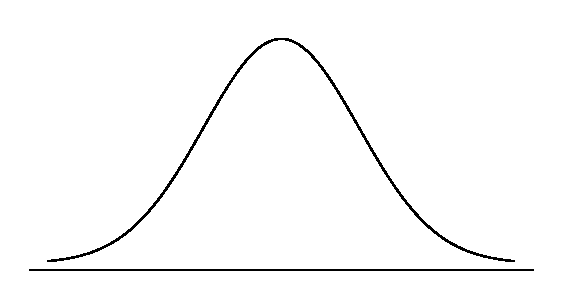
\includegraphics[scale=0.5, right]{figure/norm_draw.pdf}
\vspace{0.25cm}
\end{frame}

%----------------------------------------------
\begin{frame}[fragile]{qnorm()}
Let $Z \sim N(0,1)$ be a random variable following a standard normal distribution.  Use the R function \texttt{qnorm()} to find the value $c$ such that:\\
\begin{enumerate}[(a)]
\item $P(Z < c) = 0.025$
\item $P(Z > c) = 0.05$
\item $P(-c < Z < c) = 0.99$
\end{enumerate}
\end{frame}

%----------------------------------------------
\begin{frame}[fragile]{}
%Let $Z \sim N(0,1)$ be a random variable following a standard normal distribution.  Use the R function \texttt{qnorm()} to find the value $c$ such that:\\
%\small
\emph{Solution:}
\begin{enumerate}[(a)]
\item $P(Z<c) = 0.025$
\begin{verbatim}
> qnorm(0.025)
[1] -1.959964
\end{verbatim}
\medskip
\item $P(Z > c) = 0.05 \implies P(Z < c) = 1-0.05 = 0.95$
\begin{verbatim}
> qnorm(0.95)
[1] 1.644854
\end{verbatim}
\medskip
\item $P(-c < Z < c) = 0.99$
\begin{verbatim}
> (1 - 0.99)/2
[1] 0.005
> abs(qnorm(0.005))
[1] 2.575829
\end{verbatim}
\end{enumerate}
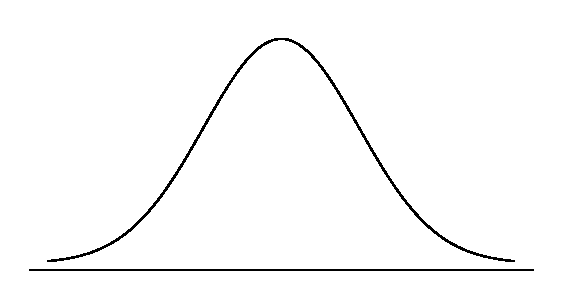
\includegraphics[scale=0.5, right]{figure/norm_draw.pdf}
\vspace{0.25cm}
\end{frame}

%----------------------------------------------
\begin{frame}[fragile]{\texttt{rnorm()}}
To generate random numbers from a normal distribution use \texttt{rnorm()}.

\begin{verbatim}
# generate 1000 random numbers from N(0,1)
> z <- rnorm(1000)
> hist(z, main='')
\end{verbatim}

\begin{figure}[htbp]
\centering
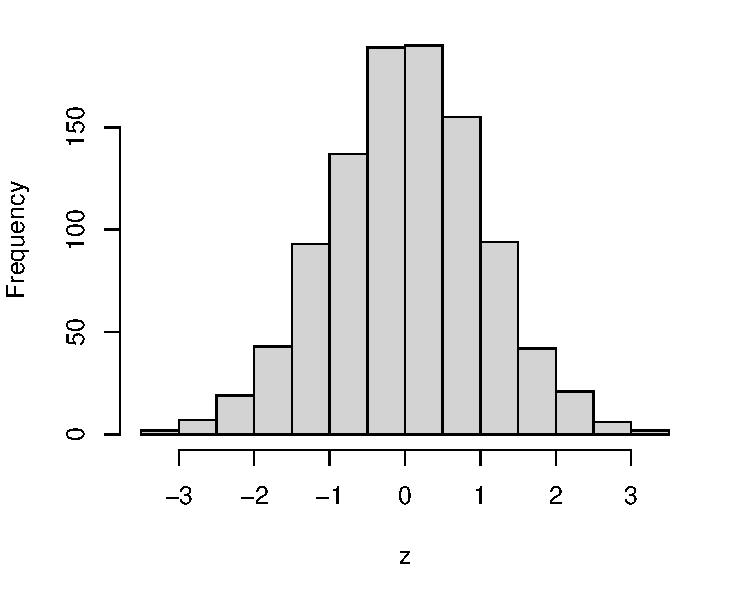
\includegraphics[scale=0.45]{figure/hist_znorm.pdf}
\end{figure}
\end{frame}

%----------------------------------------------
\begin{frame}[fragile]{}
\begin{verbatim}
# generate 1000 random numbers from N(10,3)
> x <- rnorm(1000, mean=10, sd=3)
> hist(x, main='')
\end{verbatim}

\begin{figure}[htbp]
\centering
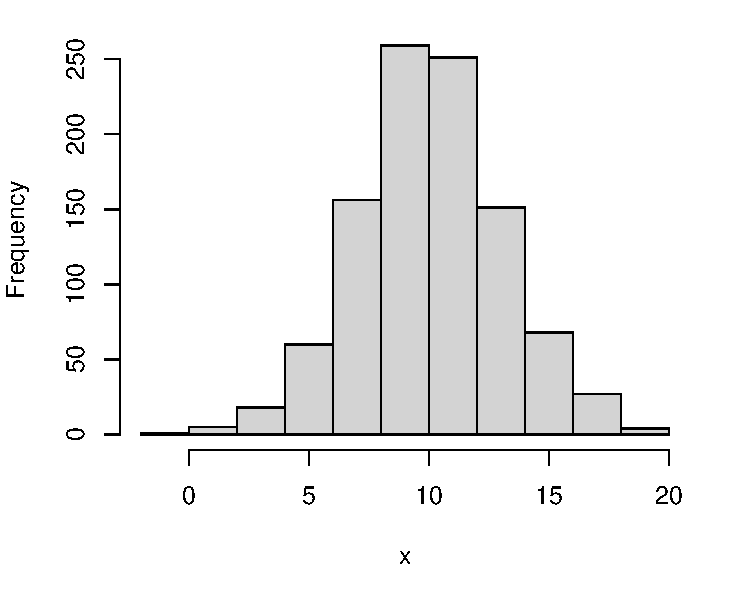
\includegraphics[scale=0.45]{figure/hist_norm1.pdf}
\end{figure}
\end{frame}

%----------------------------------------------
\begin{frame}[fragile]
Notice that each time we run \texttt{rnorm()} it produces a different set of numbers.
\small
\begin{verbatim}
> rnorm(5)
[1]  0.02252281 -0.34644394  1.06363264  0.47422096  0.38252057
> rnorm(5) # different set of numbers
[1] -0.7115876  0.1261873  0.6092906 -0.7837756 -1.0640897
\end{verbatim}
\vspace{10pt}

\normalsize
We can control this by setting a random number seed.  This will ensure the reproducibility of the results each time we run \texttt{rnorm()}.
\small
\begin{verbatim}
> set.seed(100)
> rnorm(5)
[1] -0.50219235  0.13153117 -0.07891709  0.88678481  0.11697127
> set.seed(100)
> rnorm(5) # same set of numbers
[1] -0.50219235  0.13153117 -0.07891709  0.88678481  0.11697127
\end{verbatim}
\end{frame}

%----------------------------------------------
\begin{frame}[fragile]{dnorm()}
To evaluate and plot the probability density function (pdf) for the normal distribution use \texttt{dnorm()}.  Recall that, for a normal distribution, the pdf is given by
$f(x) = \frac{1}{\sigma \sqrt{2 \pi}} e^{-\frac{1}{2} \left( \frac{x-\mu}{\sigma} \right) ^2}$

\small
\begin{verbatim}
> x <- seq(-3, 3, by=0.01)
> y <- dnorm(x)
> plot(x, y, type="l", xlab="x", ylab="f(x)", main="N(0,1)")
\end{verbatim}

\begin{figure}[htbp]
\centering
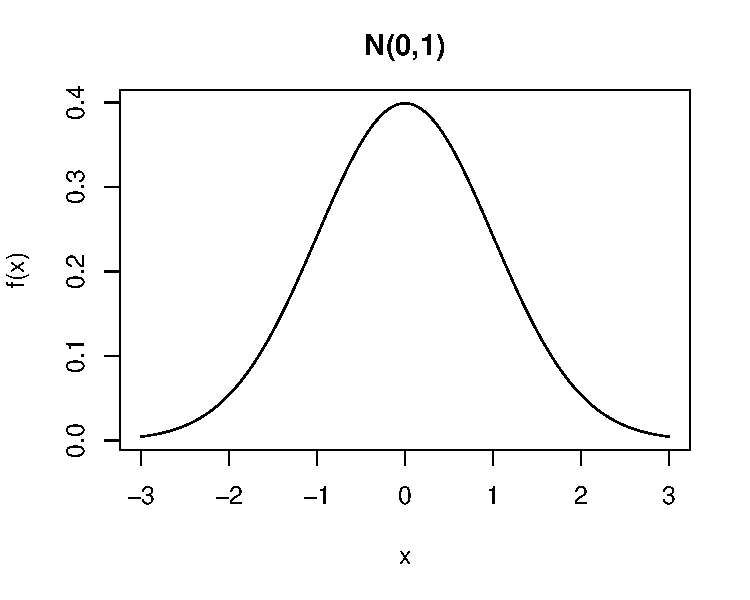
\includegraphics[scale=0.35]{figure/dnorm_z.pdf}
\end{figure}

\small
Remark: \texttt{type="l"} specifies lines instead of points in \texttt{plot()}
\end{frame}

%----------------------------------------------
\begin{frame}[fragile]
\small
\begin{verbatim}
# plot normal distribution with mean=10 and sd=3
> x <- seq(0, 20, by=0.01)
> y <- dnorm(x, mean = 10, sd = 3)
> plot(x, y, type="l", xlab="x", ylab="f(x)", main="N(10,3)")
\end{verbatim}

\begin{figure}[htbp]
\centering
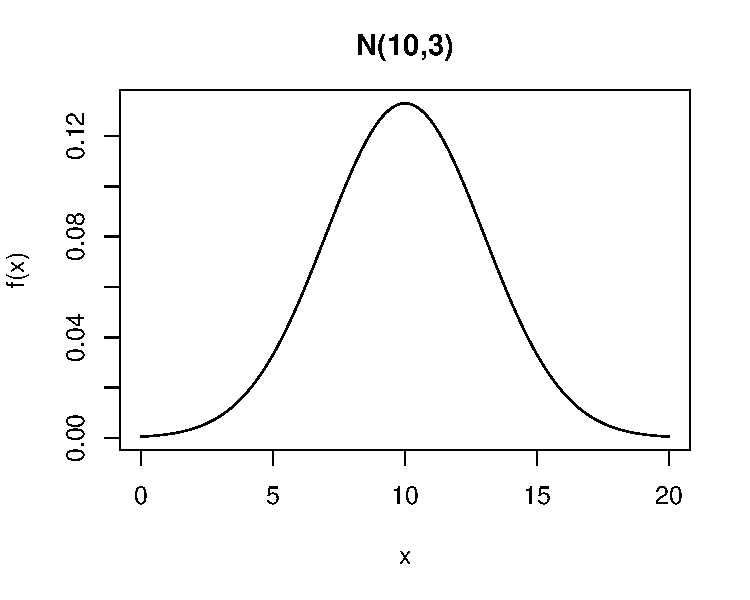
\includegraphics[scale=0.4]{figure/dnorm1.pdf}
\end{figure}
\end{frame}

%----------------------------------------------
\begin{frame}[fragile]
The \texttt{dnorm()} function is useful since it allows us to visualize how changing the parameters of the normal distribution affects the shape.  For example, the plot below shows the pdfs for the normal distribution when changing the standard deviation parameter.
\begin{figure}[htbp]
\centering
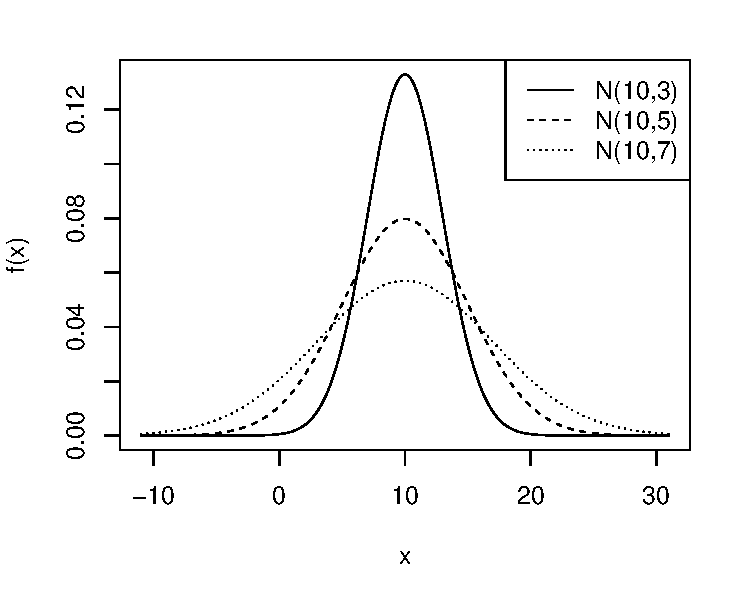
\includegraphics[scale=0.5]{figure/dnorm_sds.pdf}
\end{figure}
\end{frame}


%----------------------------------------------
\begin{frame}[fragile]
Here is the code used to make the previous figure:
\footnotesize
\begin{verbatim}
> x <- seq(-11, 31, by=0.01)
> y1 <- dnorm(x, mean = 10, sd = 3)
> y2 <- dnorm(x, mean = 10, sd = 5)
> y3 <- dnorm(x, mean = 10, sd = 7)
> 
> plot(x, y1, type="l", xlab="x", ylab="f(x)", main='')
> lines(x, y2, lty=2)
> lines(x, y3, lty=3)
> 
> legend("topright", c("N(10,3)", "N(10,5)", "N(10,7)"), lty=c(1,2,3))
\end{verbatim}

\small
Remark: The \texttt{plot()} function with \texttt{type="l"} plots the density curve for $N(10,3)$, and then the \texttt{lines()} function superimposes the other two normal density curves.  The argument \texttt{lty} specifies the different line types (solid or dashed). 
\end{frame}

%----------------------------------------------
% \begin{frame}{Your turn}
% \large
% Use \texttt{dnorm()} to plot normal density curves for the distributions $N(\mu=20, \sigma=2)$ and $N(\mu=20, \sigma=4)$.  Include both density curves on the same plot.
% \end{frame}


%----------------------------------------------
\begin{frame}{Assessing Normality}
It is important to assess whether or not a data set is approximately normally distributed.  There are two graphical methods that we will discuss:

\begin{enumerate}
\item Plotting a density histogram of the data and then superimposing a normal distribution curve.  Use the sample mean, $\bar{x}$, and sample standard deviation, $s$, as the the parameters for the ``best fitting" normal curve. 
\item A \textbf{normal probability plot}, or \textbf{normal QQ plot}, which is a plot of the sample quantiles (sorted data) on the $y$-axis, and the corresponding theoretical quantiles from the standard normal distribution on the $x$-axis.
\begin{itemize}
\item If the points follow a straight line then the data are approximately normally distributed.  Any deviations form the straight line indicate deviations in the data from the normal distribution.
\end{itemize}
\end{enumerate}
\end{frame}

%----------------------------------------------
\begin{frame}[fragile]
\scriptsize
\begin{verbatim}
> cdc <- readRDS(url("https://ericwfox.github.io/data/cdc.rds"))
> cdc_m <- subset(cdc, gender == "m") # subset males
> 
> # histogram density with normal curve
> hist(cdc_m$height, breaks=30, freq=FALSE, xlab="Male heights", main='')
> x <- seq(50, 90, 0.01)
> y <- dnorm(x, mean=mean(cdc_m$height), sd=sd(cdc_m$height))
> lines(x, y, col="red", lwd=2) 
> 
> qqnorm(cdc_m$height) # normal QQ plot
> qqline(cdc_m$height) # add line for reference
\end{verbatim}

\begin{figure}[htbp]
\centering
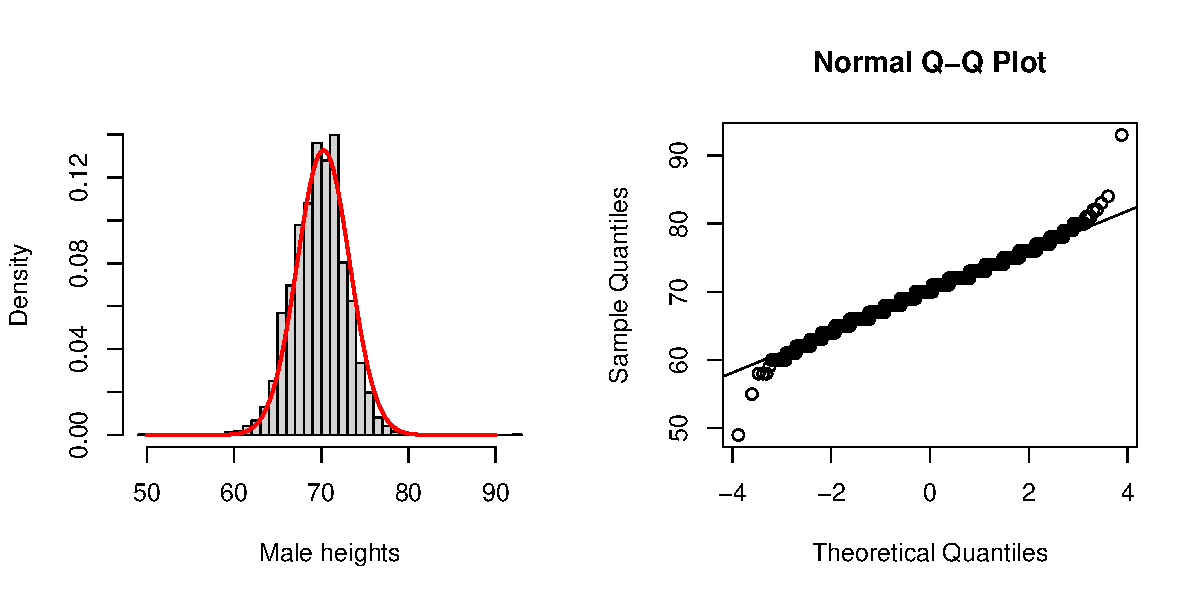
\includegraphics[scale=0.4]{figure/dhist_qq_mht.pdf}
\end{figure}

\small
Remark: The QQ plot indicates some outliers and deviations form normality in the smallest and largest values in the data set.  However, since most points fall on the line, the normal distribution model is reasonable. 
\end{frame}


%----------------------------------------------
\begin{frame}[fragile]
\scriptsize
\begin{verbatim}
> hist(cdc_m$weight, breaks=30, freq=FALSE, xlab="Male weights", main='')
> x <- seq(75, 500, 0.01)
> y <- dnorm(x, mean=mean(cdc_m$weight), sd=sd(cdc_m$weight))
> lines(x, y, col="red", lwd=2)
> 
> qqnorm(cdc_m$weight)
> qqline(cdc_m$weight)
\end{verbatim}

\begin{figure}[htbp]
\centering
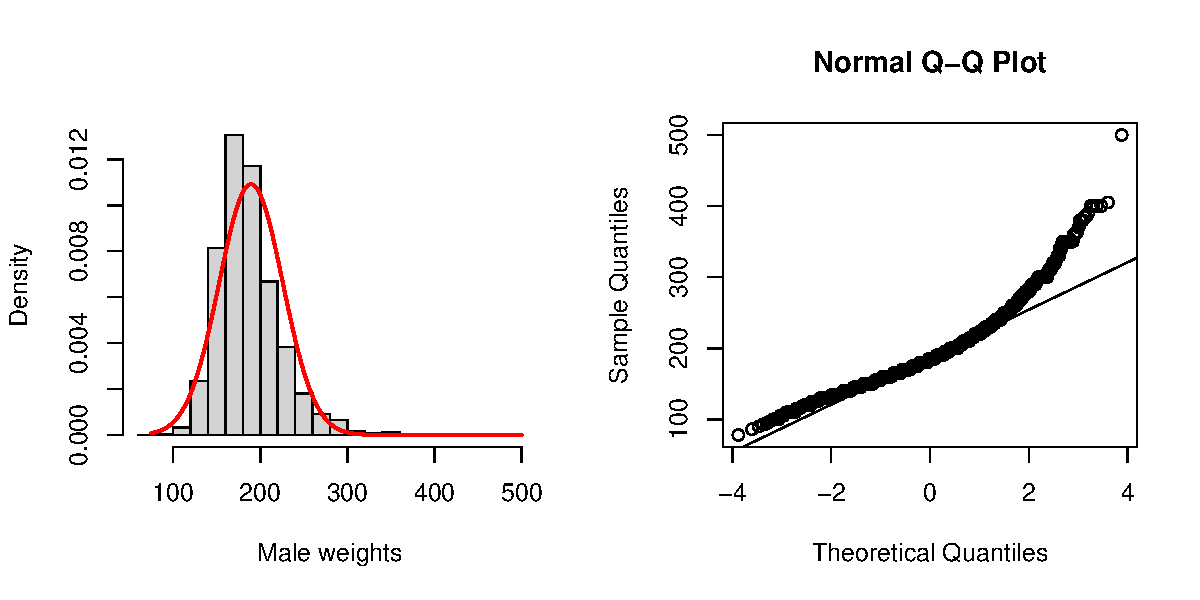
\includegraphics[scale=0.5]{figure/dhist_qq_mwt.pdf}
\end{figure}
\end{frame}

%----------------------------------------------
\begin{frame}
\begin{itemize}
\item When generating data from a normal distribution with \texttt{rnorm()} we would expect that the points in the normal probability plot follow a straight line.  \medskip
\item However, for small sample sizes it can be difficult to make a visual assessment of normality.  
 \medskip
\item In the following slides we simulate $n=30,100,1000$ values from a standard normal distribution and look at the density histograms and QQ plots. 
\end{itemize}
\end{frame}

%----------------------------------------------
\begin{frame}[fragile]
Generate $n=30$ random numbers from $N(0,1)$ and plot the density histogram and normal QQ plot.

\scriptsize
\begin{verbatim}
> set.seed(999) # set seed for reproducibility
> sim_norm30 <- rnorm(30)
> hist(sim_norm30, freq=FALSE, xlab='', main='')
> x <- seq(-3, 3, 0.01)
> y <- dnorm(x, mean=mean(sim_norm30), sd=sd(sim_norm30))
> lines(x, y, col="red", lwd=2)
> 
> qqnorm(sim_norm30)
> qqline(sim_norm30)
\end{verbatim}

\begin{figure}[htbp]
\centering
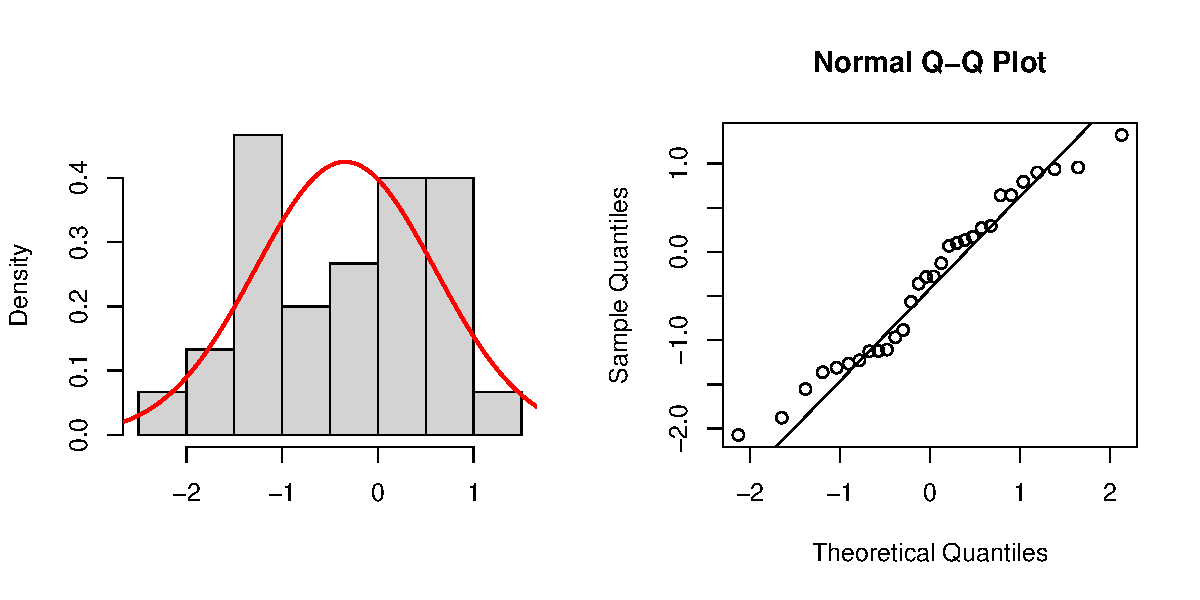
\includegraphics[scale=0.5]{figure/simnorm30.pdf}
\end{figure}
\end{frame}


%----------------------------------------------
\begin{frame}[fragile]
Generate $n=100$ random numbers from $N(0,1)$ and plot the density histogram and normal QQ plot.

\scriptsize
\begin{verbatim}
> sim_norm100 <- rnorm(100)
> hist(sim_norm100, freq=FALSE, xlab='', main='')
> x <- seq(-3, 3, 0.01)
> y <- dnorm(x, mean=mean(sim_norm100), sd=sd(sim_norm100))
> lines(x, y, col="red", lwd=2)
> 
> qqnorm(sim_norm100)
> qqline(sim_norm100)
\end{verbatim}

\begin{figure}[htbp]
\centering
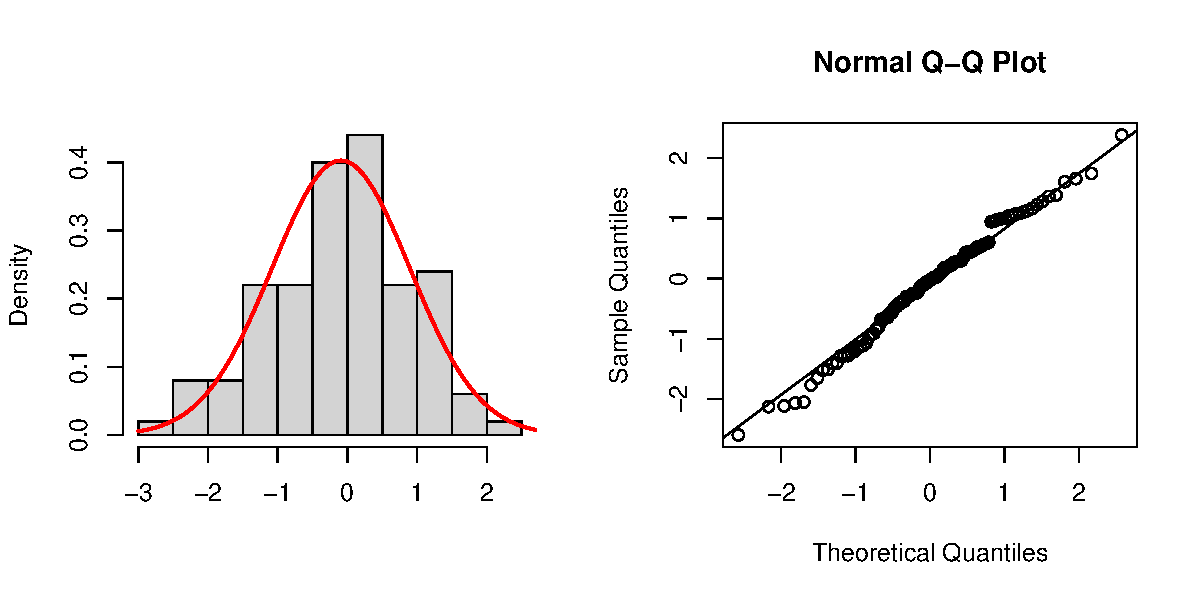
\includegraphics[scale=0.5]{figure/simnorm100.pdf}
\end{figure}
\end{frame}


%----------------------------------------------
\begin{frame}[fragile]
Generate $n=1000$ random numbers from $N(0,1)$ and plot the density histogram and normal QQ plot.

\scriptsize
\begin{verbatim}
> sim_norm1000 <- rnorm(1000)
> hist(sim_norm1000, freq=FALSE, xlab='', main='')
> x <- seq(-3, 3, 0.01)
> y <- dnorm(x, mean=mean(sim_norm1000), sd=sd(sim_norm1000))
> lines(x, y, col="red", lwd=2)
> 
> qqnorm(sim_norm1000)
> qqline(sim_norm1000)
\end{verbatim}

\begin{figure}[htbp]
\centering
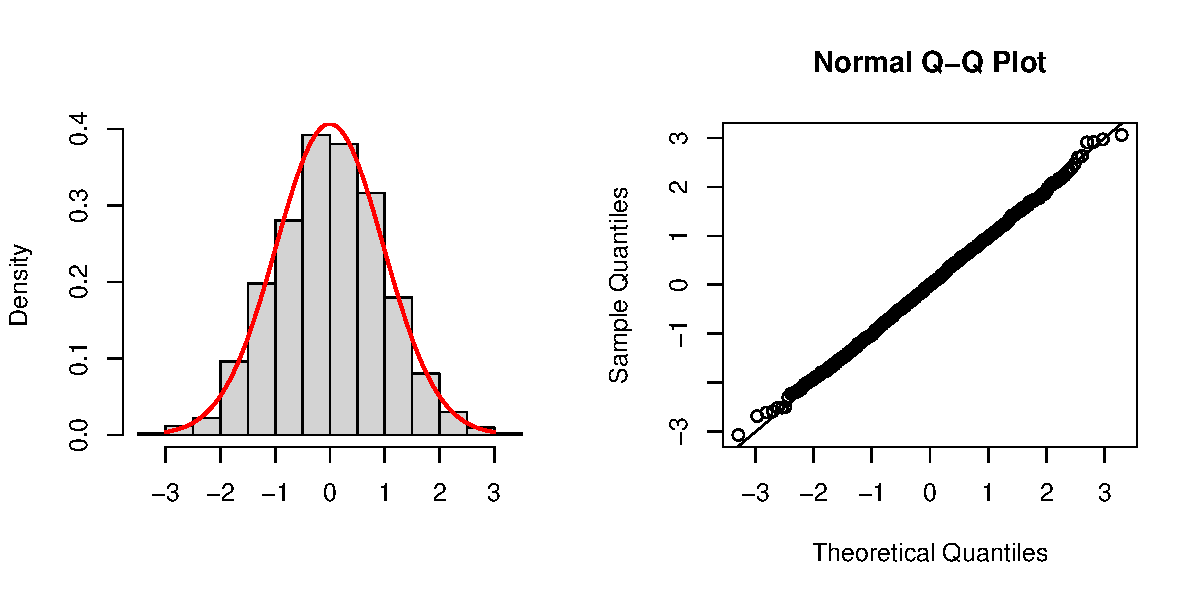
\includegraphics[scale=0.5]{figure/simnorm1000.pdf}
\end{figure}
\end{frame}

% \begin{frame}{Interpreting QQ-plots}
% \begin{figure}[htbp]
% \centering
% 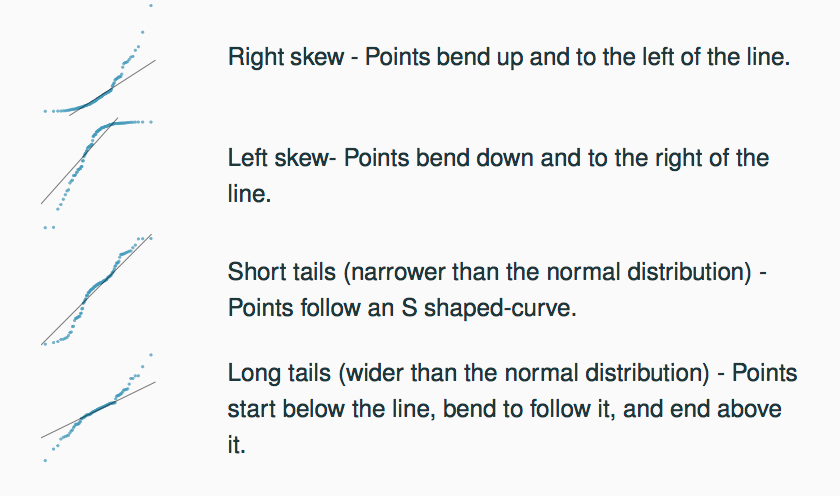
\includegraphics[width=\textwidth]{figure/qqplot_interpret.png}
% \end{figure}
% \small
% Figure from \url{https://www.openintro.org}.
% \end{frame}

%----------------------------------------------
\begin{frame}{References}
If you would like to read more about normal probability plots the following are good references:
\begin{itemize}
\item Chihara and Hesterberg. \emph{Mathematical Statistics with Resampling and R}, 4th edition, Section 2.4.
\item \url{https://www.itl.nist.gov/div898/handbook/eda/section3/normprpl.htm}
\item \url{https://en.wikipedia.org/wiki/Normal_probability_plot}\\
\end{itemize}
\vspace{10pt}

You can also use the R help menu to read more about \texttt{dnorm()}, \texttt{pnorm()}, \texttt{qnorm()}, and \texttt{rnorm()}
\end{frame}

\end{document}